\section{Bases Reducidas hp Greedy}

El nombre del método hp greedy viene de la combinación del \textit{``refinamiento p''} y del \textit{``refinamiento h"}. El \textit{refinamiento p} proviene de los métodos espectrales con bases polinomiales \cite{hesthaven_gottlieb_gottlieb_2007} y se refiere a la propiedad de que el error de representación disminuye al aumentar el grado del polinomio (en el caso de las bases reducidas aumenta el número de elementos en la base). Por otro lado el término de \textit{refinamiento h} se toma prestado de los métodos de diferencias finitas, donde el tamaño de cada celda de la grilla es representado por \textit{h}. En este caso el refinamiento ocurre en el espacio de los parámetros (y no en el dominio físico).

\subsection{Refinamiento h}

Partiendo de la siguiente notación:
\begin{itemize}
\item $V$: espacio de parámetros para un dado subdominio $D$.
\item $V_1, V_2$ : particiones de $V$.
\item $\Lambda_V$ : parámetros \textit{greedy} para $V$.
\item  $\hat{\Lambda}_{V}$: punto de anclaje para $V$.
%\item  $\hat{\Lambda}_{V_1}, \hat{\Lambda}_{V_2}$
\end{itemize}

El refinamiento en el dominio de los parámetros ocurre a partir de la división recursiva de cada subdominio $V$ del dominio total $D$ en dos subdominios $V_1$ y $V_2$. De forma que se obtiene una estructura de árbol binario.


Esta descomposición binaria del dominio está descrita en forma de pseudocódigo en el algoritmo \ref{alg:part}.

Al algoritmo ingresan tres objetos:

\begin{itemize}
\item $\lambda_V$: conjunto de parámetros resultado de un muestreo de $V$.
\item $\hat{\Lambda}_{V_1}, \hat{\Lambda}_{V_2}$: puntos de anclaje (son los primeros dos elementos de $\Lambda_V$).
\end{itemize}

Luego, para cada parámetro del conjunto $\lambda_V$ se evalúa su distancia a los puntos de anclaje a partir de la \textit{función de proximidad} $d: d(\lambda_1, \lambda_2)$:

\[
d(\lambda_1, \lambda_2) = ||\lambda_1 - \lambda_2||_2,
\]

de forma que se obtengan dos conjuntos; $\lambda_{V_1}$ con los $\lambda_{i}$ más proximos a $\hat{\Lambda}_{V_1}$, y $\lambda_{V_2}$ con los $\lambda_{i}$ más proximos a $\hat{\Lambda}_{V_2}$, tal que  $\lambda_{V} =\lambda_{V_1} \cup \lambda_{V_2}$. Este resultado es la división del espacio de parámetros a partir de los puntos de anclaje.

\begin{algorithm}
\caption{\texttt{Partition}\((\lambda_V, \hat{\Lambda}_{V_1}, \hat{\Lambda}_{V_2})\)}\label{alg:part}
\begin{algorithmic}[1]
\Require $\lambda_V, \hat{\Lambda}_{V_1}, \hat{\Lambda}_{V_2}$ 
\vspace{3mm}
\State $\lambda_{V_1} = \lambda_{V_2} = \emptyset$
\For{\textbf{each} $\lambda_i \in \lambda_V$}
	\If{$d(\lambda_i, \hat{\Lambda}_{V_1}) <d(\lambda_i, \hat{\Lambda}_{V_2})$}
		\State $\lambda_{V_1} = \lambda_{V_1} \cup \lambda_i$
	\ElsIf{$d(\lambda_i, \hat{\Lambda}_{V_1}) >d(\lambda_i, \hat{\Lambda}_{V_2})$}
		\State $\lambda_{V_2} = \lambda_{V_2} \cup \lambda_i$
	\Else
		\State $\lambda_{V'} = $ random choice$([\lambda_{V_1}, \lambda_{V_2}])$
		\State $\lambda_{V'} = \lambda_{V'} \cup \lambda_i$
	\EndIf
\EndFor
\vspace{3mm}
\Ensure $\lambda_{V_1}, \lambda_{V_2}$
\end{algorithmic}
\end{algorithm}

\subsection{Refinamiento hp-greedy}


El refinamiento hp-greedy es un método que combina el algoritmo greedy para la construcción de bases reducidas con la partición del dominio de parámetros. 

Esta partición recursiva del dominio de parámetros da lugar a una estructura de árbol binario, la cual tendrá diferentes niveles $l$ de profundidad, con un $l_{max}$ establecido por el usuario, de forma que $l : 0 \le l \le l_{max}$, donde $l =0$ es el nodo raíz. Cada nodo del árbol estará etiquetado por un conjunto de índices $B_l$, que parte de:

\[
B_0 = (0,),
\]
luego sus dos hijos ($l=1$) tendrán las etiquetas:
\[
B_1 = (0,0,) \ \ o \ \  (0, 1, ),
\]
y en general:
\[
B_l = (0, i_1, \cdots, i_l), \ \  con \ \ i_j = \{0, 1\},
\]

\noindent donde cada nivel $l$ tendrá un máximo de $2^l$ nodos.
Los nodos que no tengan hijos se llamarán nodos \textit{hojas}.
\begin{figure}[h!]
\centering
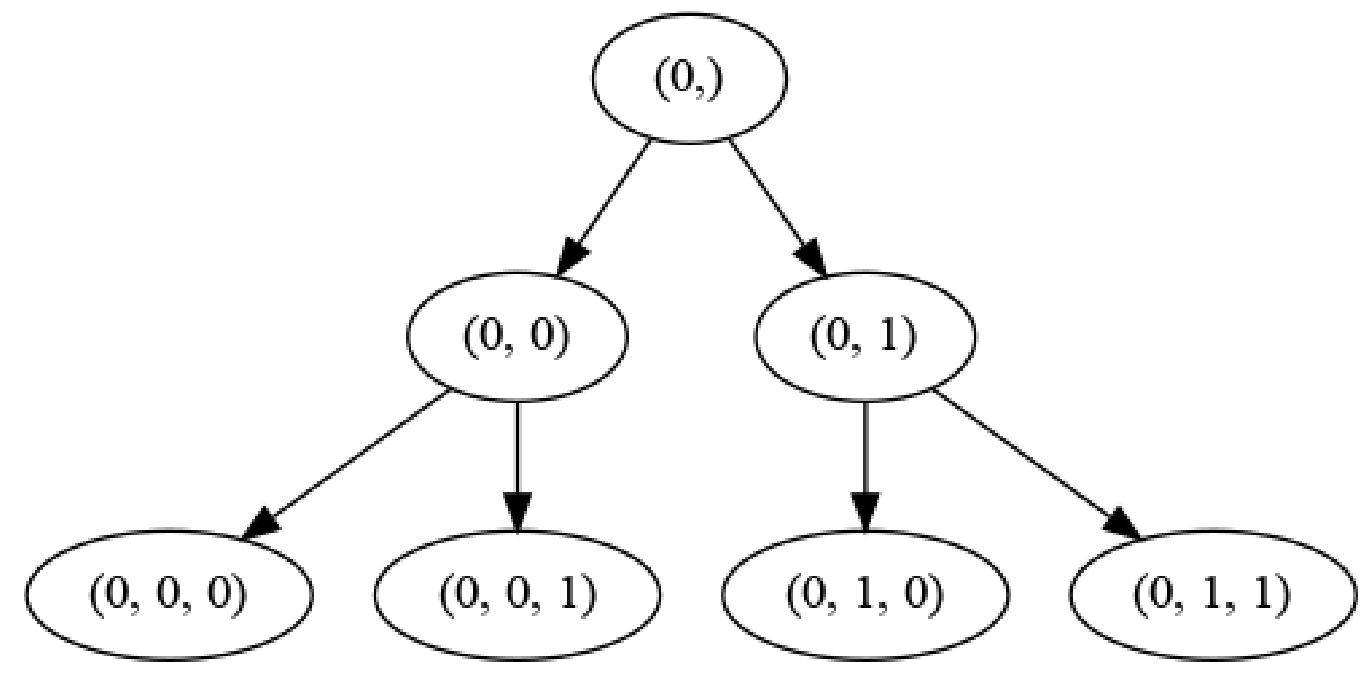
\includegraphics[width=.5\columnwidth]{Bl_lmax2.png}
\caption{Representación de los nodos de un árbol con $l_{max}=2$.}
\end{figure}

El método está explicado en el algoritmo \ref{alg:hp}; partiendo de un dado dominio de parámetros $V$ se construye una base reducida a partir de un conjunto de entrenamiento $\mathcal{T}_V = \{h_{\lambda_{V_i}}\}_{i=1}^{N}$, una \textit{tolerancia greedy} $\varepsilon$ y un $n_{max}$ (para esto se utiliza el algoritmo \textbf{[VERIFICAR REFERENCIA]}). Si el error de representación $\sigma$ es mayor que la tolerancia $\varepsilon$, y si la profundidad del nivel $l$ es menor a $l_{max}$, entonces se realizará una partición del dominio $V$ utilizando como puntos de anclaje a los dos primeros parámetros \textit{greedy}. En cada dominio se realizará el mismo procedimiento hasta que se cumpla que $l = l_{max}$ o hasta que $\sigma \le \varepsilon$.

 % El conjunto $\lambda_V$ representa el conjunto de parámetros de $\mathcal{T}_V$

\begin{algorithm}
\caption{\texttt{hpGreedy}\((\mathcal{T}_V, \lambda_V, \varepsilon, n_{max}, l, l_{max}, B_{l})\)}\label{alg:hp}
\begin{algorithmic}[1]
\Require $\mathcal{T}_V, \lambda_V, \varepsilon, n_{max}, l, l_{max}, B_{l}$ 
\vspace{3mm}
\State rb, $\Lambda_V$, $\sigma$ = \texttt{GreedyRB}($\mathcal{T}_V,\lambda_V, \varepsilon, n_{max}$) 
\vspace{3mm}
\If{$\sigma > \varepsilon$ \textbf{and} $l<l_{max}$}
	\State $\hat{\Lambda}_{V_1} = \Lambda_V[1]$
	\State $\hat{\Lambda}_{V_2} = \Lambda_V[2]$
	\State $\lambda_{V_1}, \lambda_{V_2} =$ \texttt{Partition}$(\lambda_V,\hat{\Lambda}_{V_1}, \hat{\Lambda}_{V_2})$
	\State $out_1 = $ \texttt{hpGreedy}\((\mathcal{T}_{V_1}, \lambda_{V_1}, \varepsilon, n_{max}, l+1, l_{max}, (B_{l}, 0))\)
	\State $out_2 = $ \texttt{hpGreedy}\((\mathcal{T}_{V_2} ,\lambda_{V_2}, \varepsilon, n_{max}, l+1, l_{max}, (B_{l}, 1))\)
	\State $out = out_1 \cup out_2$
\Else
	\State $out = \{( rb, \Lambda_V, B_l)\}$
\EndIf
\vspace{3mm}
\Ensure out
\end{algorithmic}
\end{algorithm}

El resultado del algoritmo \ref{alg:hp} es una estructura arbórea, donde cada nodo contiene la información de sus puntos de anclaje, por lo que en el caso de querer proyectar un conjunto de validación, cada onda gravitacional se proyectará a la base reducida del nodo hoja con el punto de anclaje más cercano al parámetro de la onda.


\subsection{Aplicación a Ondas Gravitacionales}

Se trabaja a partir de un conjunto de ondas gravitacionales con parámetro bidimensional, donde $\chi_{1_z} = \chi_{2_z} = \chi_z$, es decir que $\lambda = (q, \chi_z)$. De esta forma se puede graficar fácilmente el dominio de parámetros.



En la figura \ref{fig:part1} se puede observar una representación de la partición del dominio de parámetros. En la primera imagen se pueden ver los dos puntos de anclaje, que son los primeros dos elementos de la base global construida inicialmente. En cada nueva división se construye una nueva base global con la cual se realiza la siguiente partición de cada subdominio.


\begin{figure}[h!]
\centering
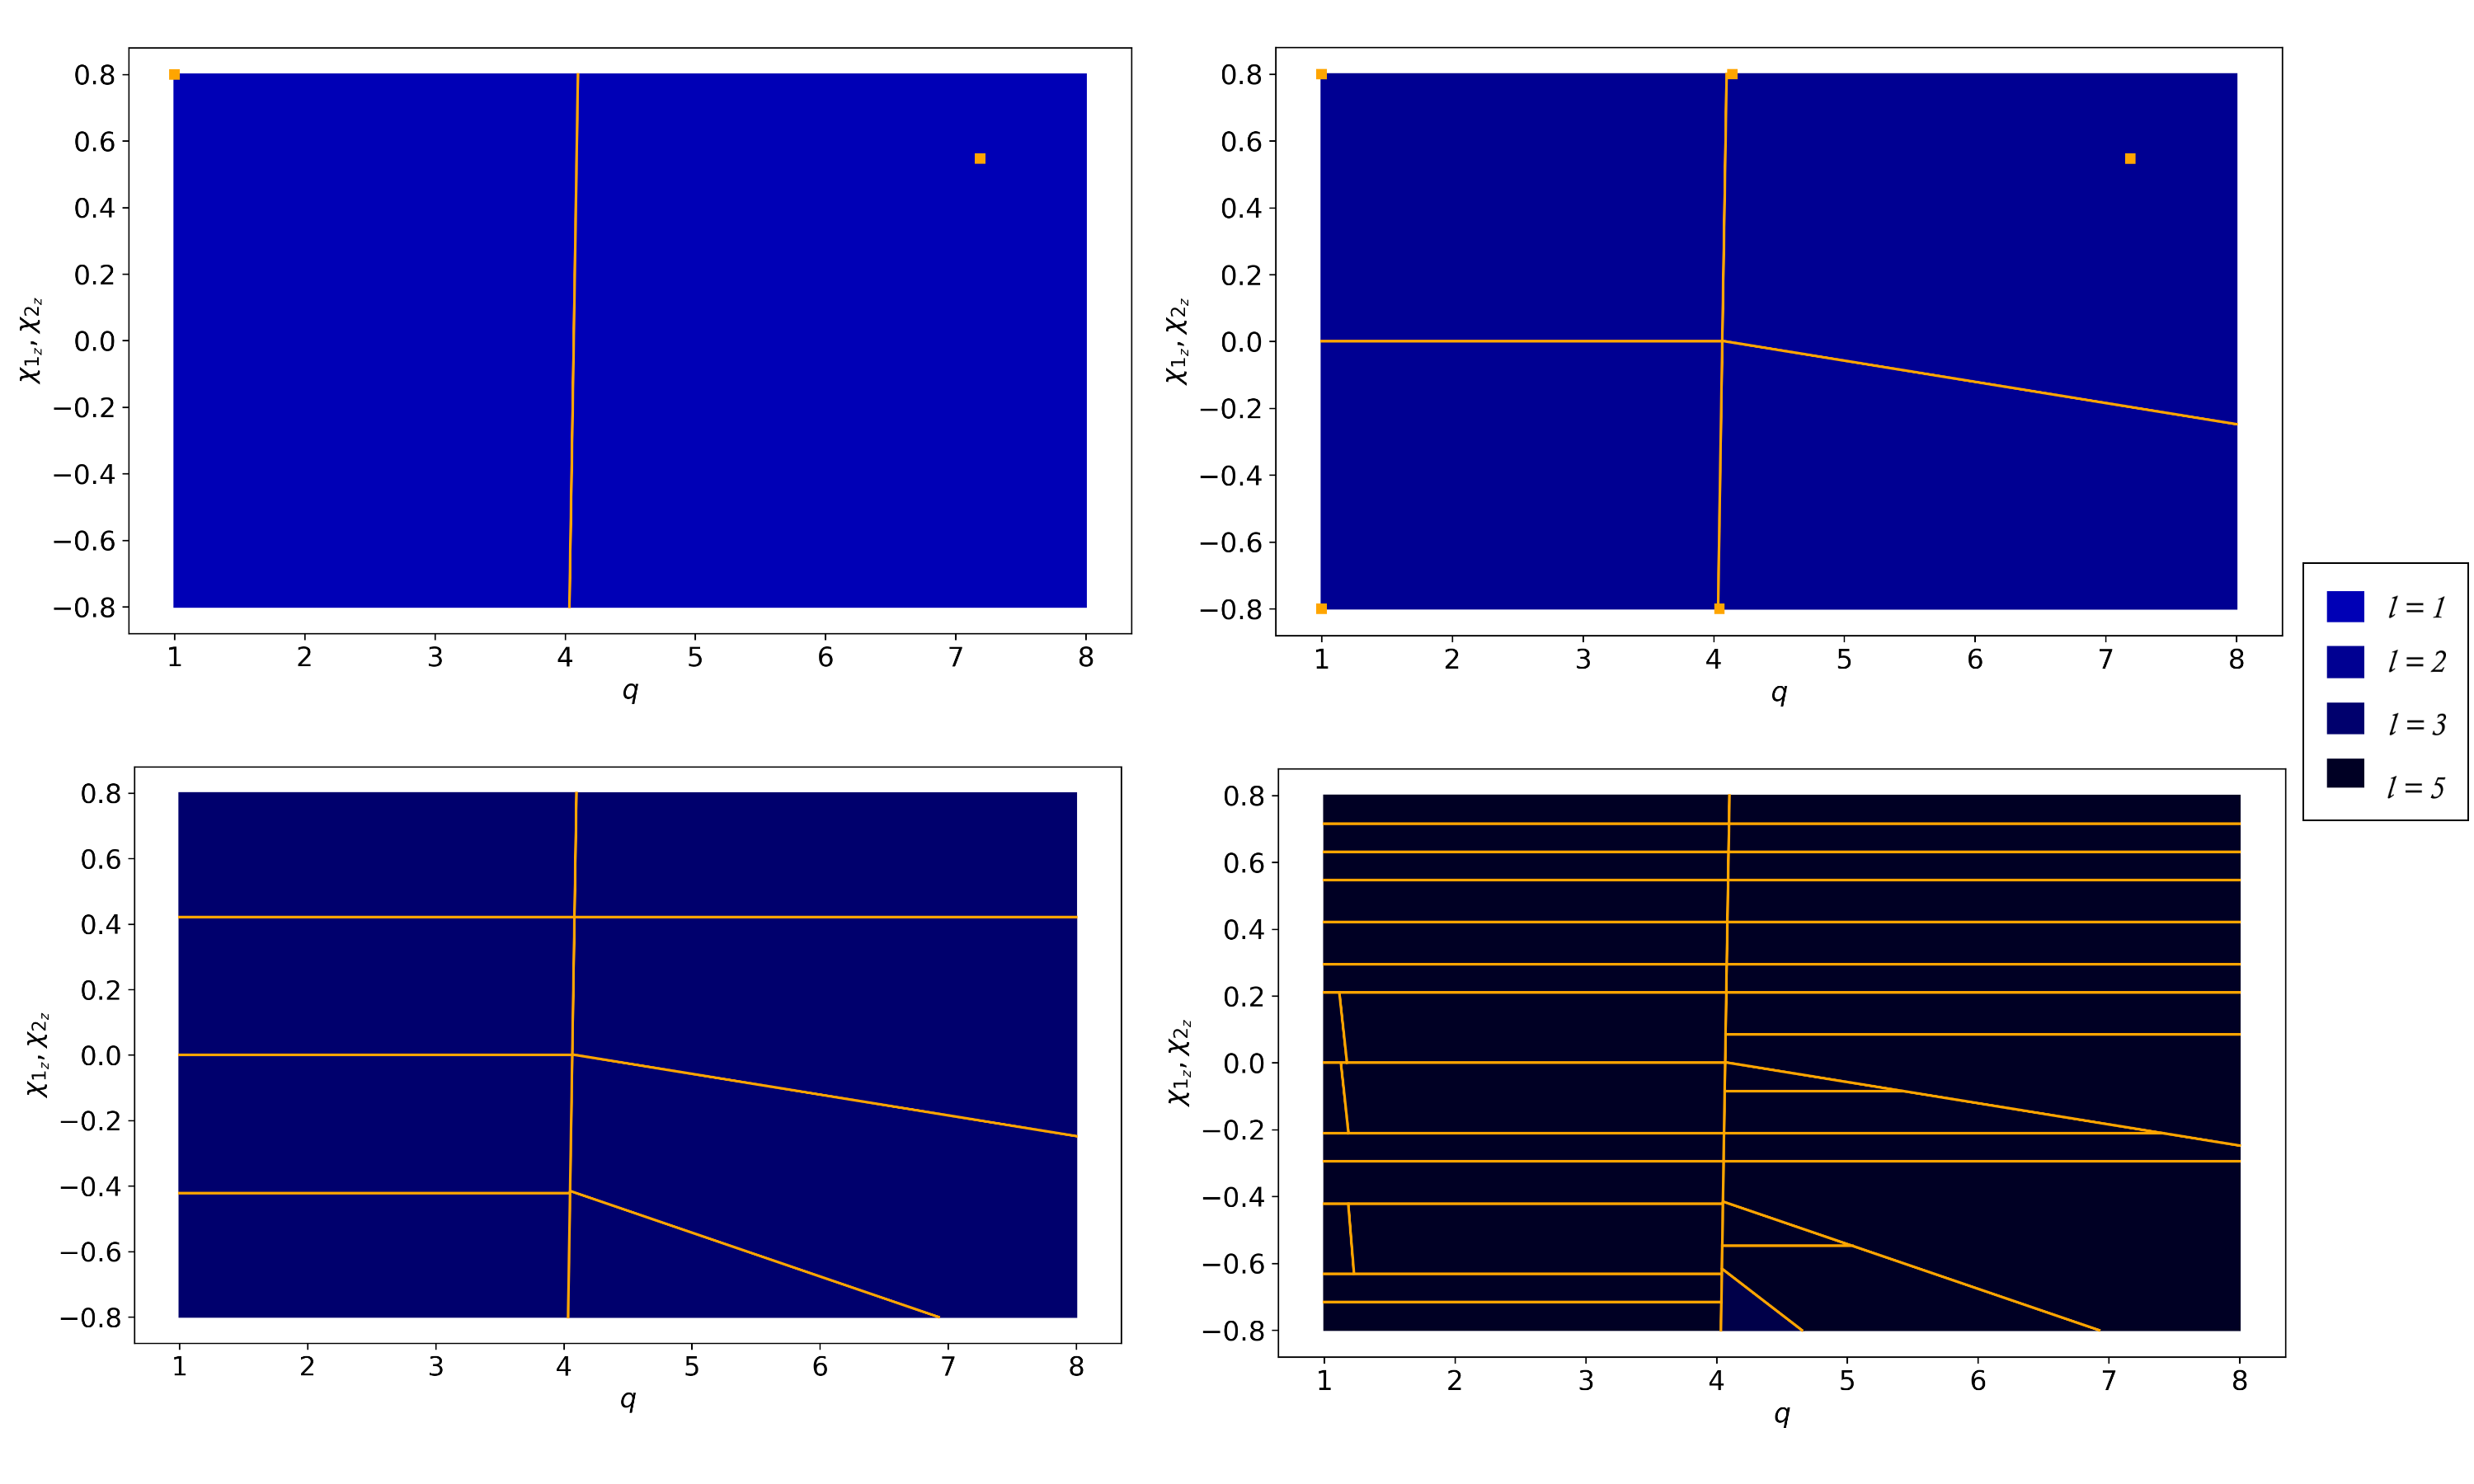
\includegraphics[width=1\columnwidth]{figs/particion2d.png}
\caption{Ejemplo de partición del espacio de parámetros bidimensional para $l_{max}= 1, 2, 3$ y $5$. En los primeros dos casos se muestran los puntos de anclaje.}
\label{fig:part1}
\end{figure}


En la figure \ref{fig:l0vl4} se compara el máximo error de representación obtenido para un conjunto de validación con una base global, es decir, con $l_{max} = 0$, y con $l_{max}=4$. La velocidad de convergencia es claramente mayor en el segundo caso.

\begin{figure}[h!]
\centering
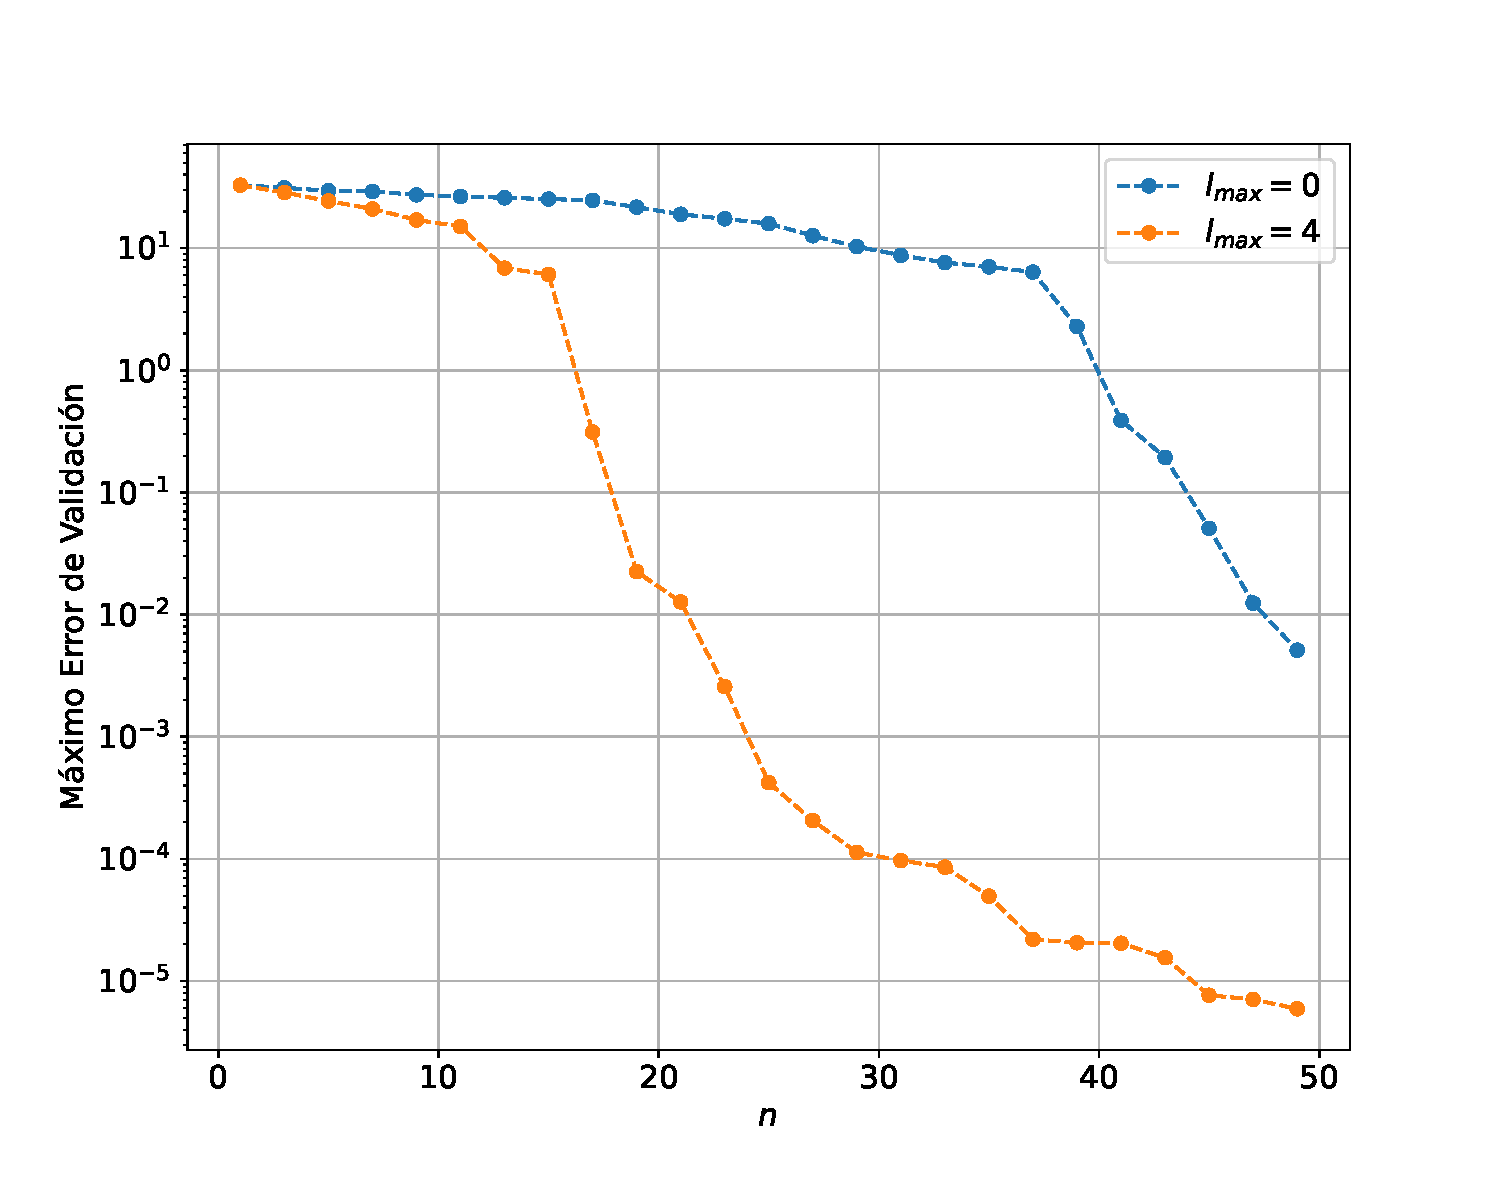
\includegraphics[width=.8\columnwidth, trim={0, 1.3cm, 0, 1.4cm}]{figs/l0vsl4.pdf}
\caption{Base global ($l_{max} = 0$) versus base con $l_{max} = 4$} para distintos valores de $n$.
\label{fig:l0vl4}
\end{figure}


El aspecto más importante de este método es que permite disminuir la complejidad temporal del algoritmo a la hora de proyectar la base, a cambio de aumentar la complejidad espacial, pues si bien cada subdominio tendrá un máximo de $n_{max}$ elementos en su base, habrá un máximo de $2^{l_{max}}$ subdominios.

\begin{figure}[h!]
\centering
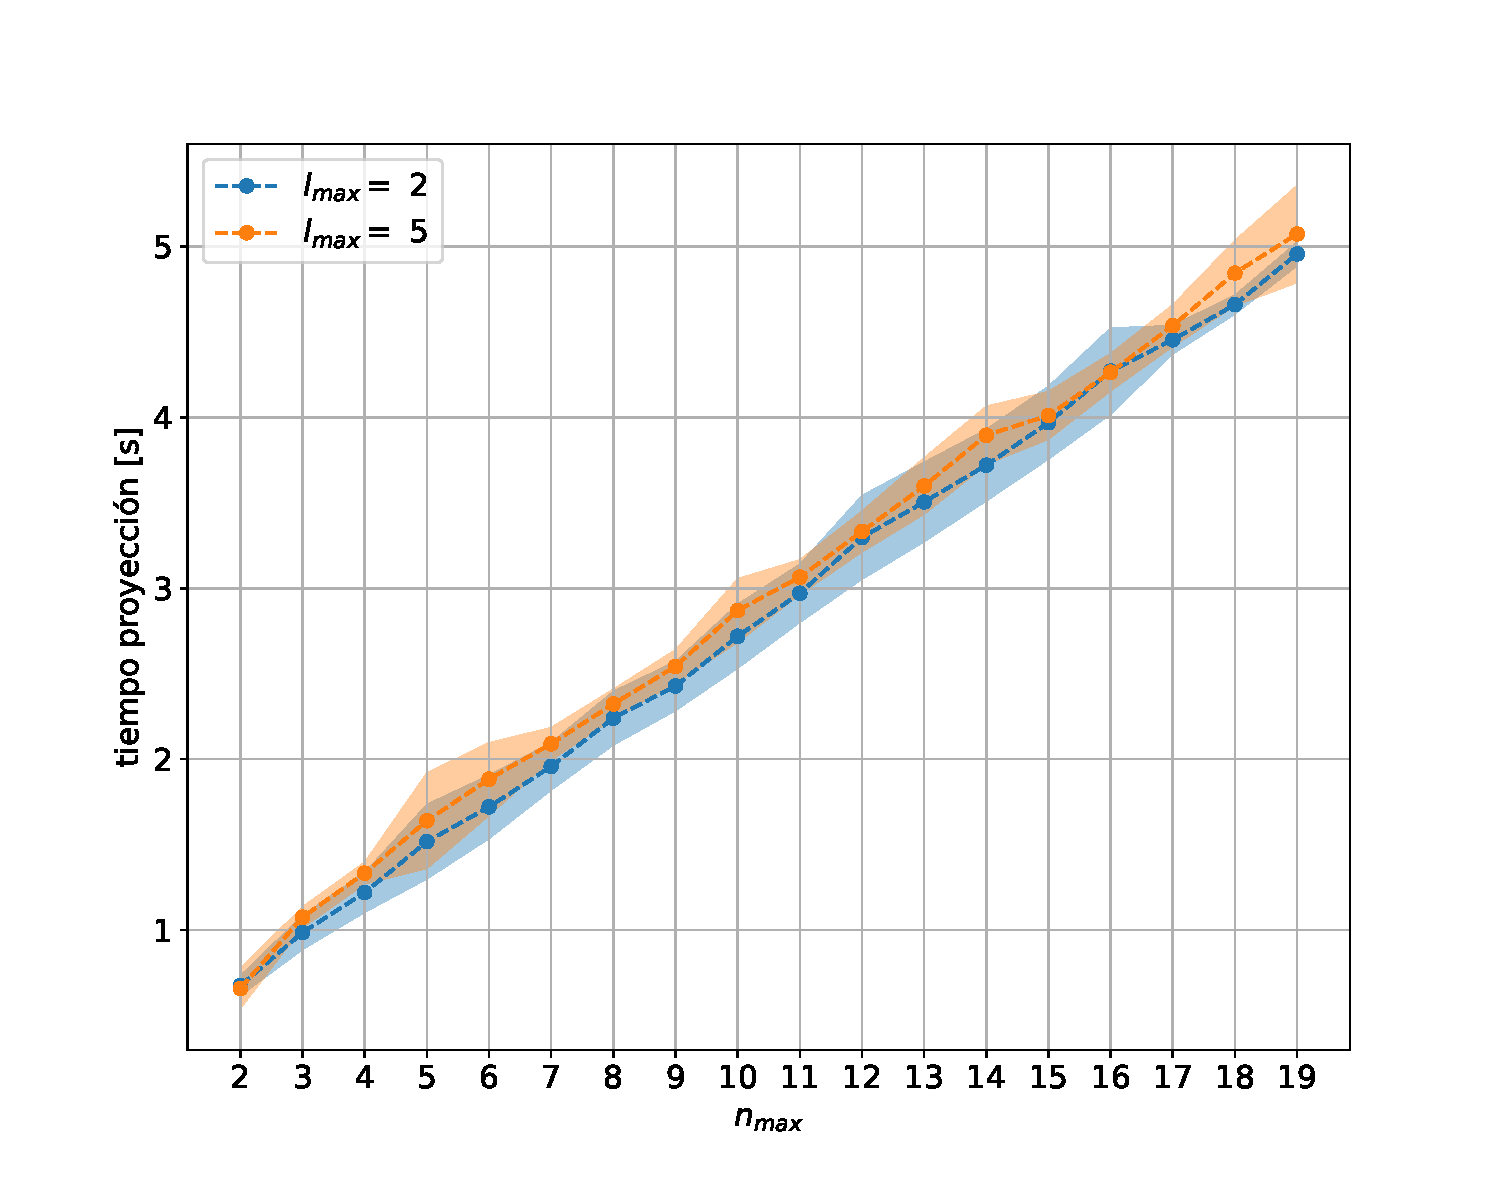
\includegraphics[width=.8\columnwidth ,trim={0, 1cm, 0, 1.2cm}]{figs/t_vs_nmax.pdf}
\caption{tiempos de proyección de un conjunto de validación a dos bases con distinto $l_{max}$ en función del $n_{max}$. En cada caso la linea de trazo representa el valor medio, y el área de color indica una desviación estandar desde el valor medio, para cada medición.}
\label{fig:t_vs_nmax}
\end{figure}


En la figura \ref{fig:t_vs_nmax} se graficó el tiempo de proyección de un conjunto de validación a dos bases \textit{hp-greedy} con distinto valor de $l_{max}$. Se observa que el tiempo es bastante lineal en relación al $n$ (elementos de las bases locales), y no parece ser afectado por $l_{max}$.



\begin{figure}[h!]
\centering
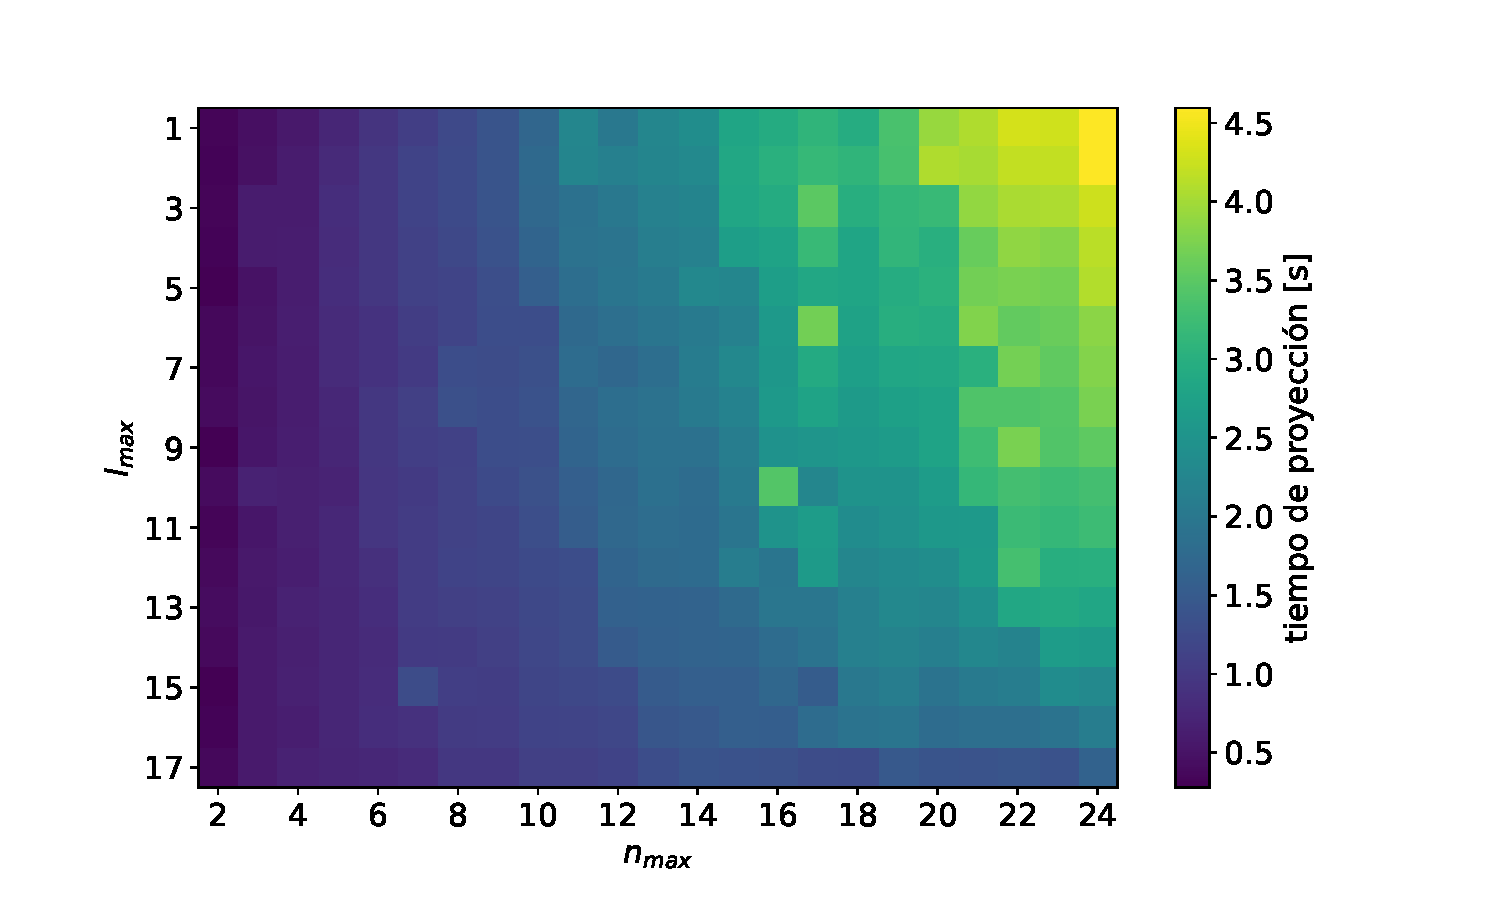
\includegraphics[width=.9\columnwidth, trim={0, 1cm, 0, 1.4cm}]{figs/nmax_lmax_t_grid.pdf}
\caption{Tiempo de proyección de un conjunto de validación para diferentes valores de $n_{max}$ y $l_{max}$}
\label{fig:t_grilla_nl}
\end{figure}


En la figura \ref{fig:t_grilla_nl} se puede ver el tiempo de proyección para más valores de $n_{max}$ y ${l_max}$. En los primeros valores de $l_{max}$ se observa un comportamiento similar al descrito anteriormente, donde el tiempo depende casi únicamente de $n_{max}$. Sin embargo al aumentar el $l_{max}$ se observa que el tiempo disminuye. Esto se puede entender en dos partes:

\begin{itemize}
\item \textbf{Independencia aparente entre el tiempo de proyección y $l_{max}$}: para realizar la proyección de cada onda del conjunto de validación en la base \textit{hp-greedy} primero se debe buscar el subdominio (la hoja) correspondiente utilizando los puntos de anclaje de la estructura arbórea de la base. Luego se proyectará la onda en la base local del subdominio en cuestión. Si bien la búsqueda en el árbol tiene una complejidad temporal $O(l_{max})$, el trabajo de cómputo más importante es el que se realizará al momento de proyectar la base, que es independiente de $l_{max}$, con una complejidad temporal $O(n_{max})$. Pero esto solo se cumple hasta ciertos valores de $l_{max}$.
\item \textbf{Disminución del tiempo de proyección al aumentar $l_{max}$}: ya se mencionó en más de una ocasión que por cada nivel $l$ hay un máximo de $2^l$ subdomínios. Es decir que si se quiere obtener el número de elementos de todas las bases en las hojas del árbol, suponiendo un árbol denso, este número será $n_{max} \times 2^{l_{max}}$. En la figura \ref{fig:t_grilla_nl} se utilizó un conjunto de entrenamiento con 1400 ondas, por lo que al llegar a unos valores de $l_{max} = 6$ y $n_{max} = 24$ en total debería haber 1536 elementos de base en total. Es decir, más elementos de base que ondas en el conjunto de entrenamiento. Por lo tanto al aumentar el $l_{max}$ rápidamente se aumenta el número de subdominios, reduciendo su tamaño como resultado y reduciendo el número de elementos de las bases locales (cada subdominio tendrá una cantidad de elementos menor a $n_{max}$). De esta forma se explica la disminución del tiempo de proyección para valores grandes de $l_{max}$, consecuencia del tamaño limitado del conjunto de entrenamiento.
\end{itemize}


\subsection{Hiperparámetros}

\begin{figure}[h!]
\centering
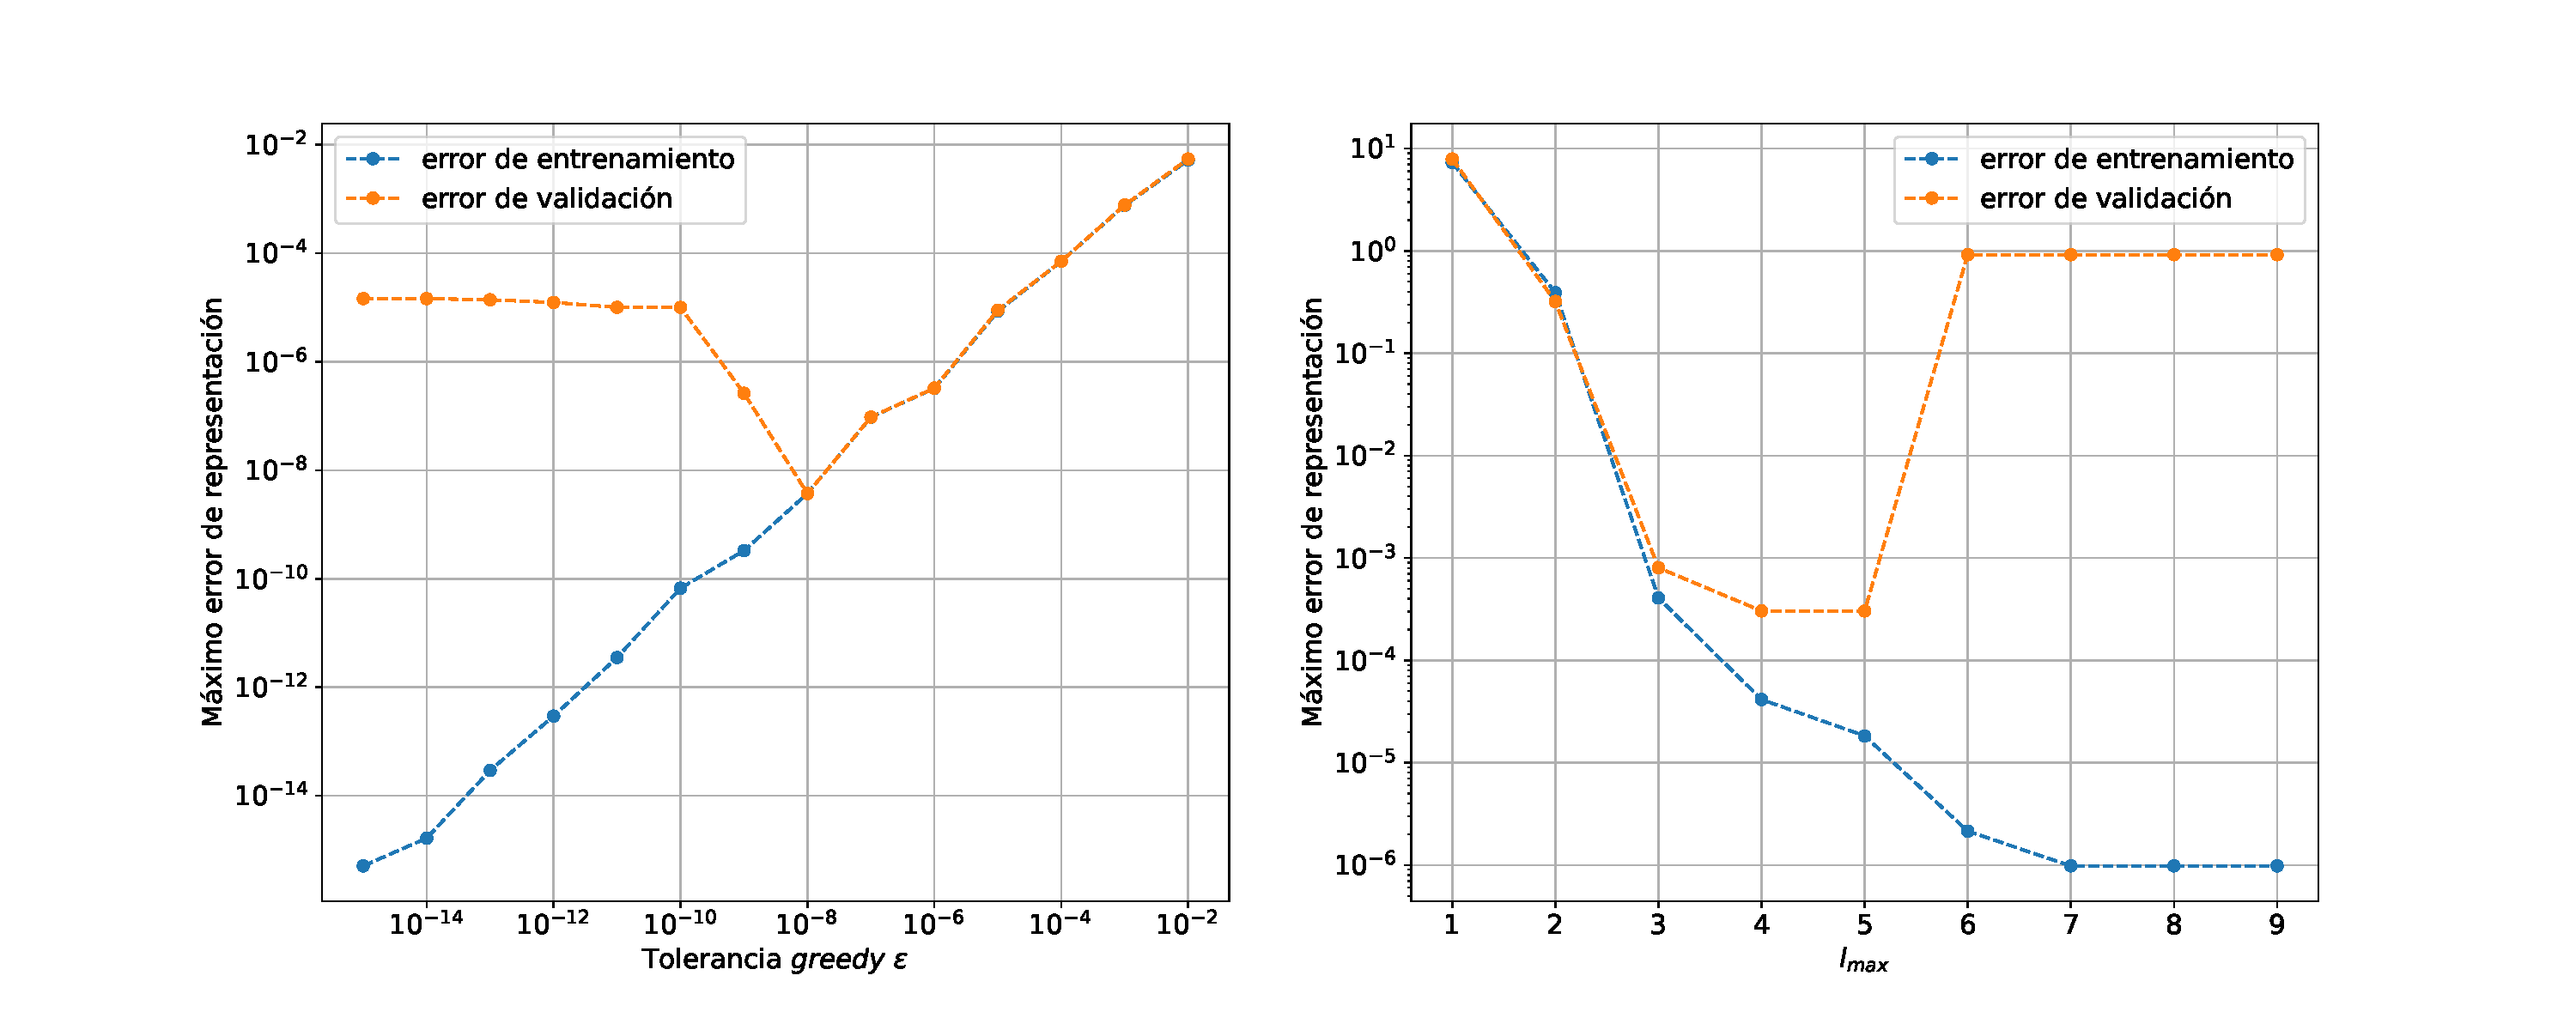
\includegraphics[width=1\columnwidth ,trim={2cm, 1cm, 1cm, 1.2cm}]{figs/overfit.pdf}
\caption{Ejemplos de \textit{sobreajuste}. A la izquierda variando $\varepsilon$ con $(n_{max}, l_{max}) = (25, 19)$ en un conjunto de parámetro unidimensional $(\lambda_i = q_i)$. A la derecha variando $l_{max}$ con $(n_{max}, \varepsilon) = (20, 1\times10^{-6})$ en un conjunto de parámetro bidimensional$(\lambda_{ij} = (q_i, \chi_{z_j})) $.}
\label{fig:overfit}
\end{figure}

Al momento de construir una base \textit{hp-greedy} entran en juego cuatro hiperparámetros. Los primeros tres son los parámetros de parada;
\begin{itemize}
\item $\bm{n_{max}}:$ determina la cantidad máxima de elementos para cada base local. A mayor cantidad de elementos el error de representación será menor, pero el tiempo requerido para proyectar un conjunto de validación a la base depende casi exclusivamente de este hiperparámetro.
\item $\bm{l_{max}}:$ determina la máxima profundidad de las hojas del árbol. En general al aumentar $l_{max}$ disminuye el error de representación, pero valores muy elevados junto a cierta combinación de hiperparámetros pueden dar lugar a sobreajustes en el modelo, un ejemplo de esto se puede ver en la figura \ref{fig:overfit}. Este es un comportamiento típico de las estructuras arbóreas.
\item $\bm{\varepsilon}$: la tolerancia \textit{greedy} interviene tanto en el tamaño de las bases locales como en la profundidad de las hojas del árbol. Un valor de $\varepsilon$ demasiado bajo también puede dar lugar a sobreajuste, sobre todo con valores muy altos de $l_{max}$. Un valor de $\varepsilon = 0$ implica que se obtiene un árbol totalmente denso, determinado únicamente por $n_{max}$ y $l_{max}$, y al aumentar el valor de $\varepsilon$ se puede pensar en la analogía de podar un árbol, de forma que se previene el sobreajuste.
\end{itemize}

Al cuarto hiperparámetro se le da el nombre de \textit{\textbf{semilla}} y se la denota con $\bm{\hat{\Lambda}_0}$;

\begin{figure}[h!]
\centering
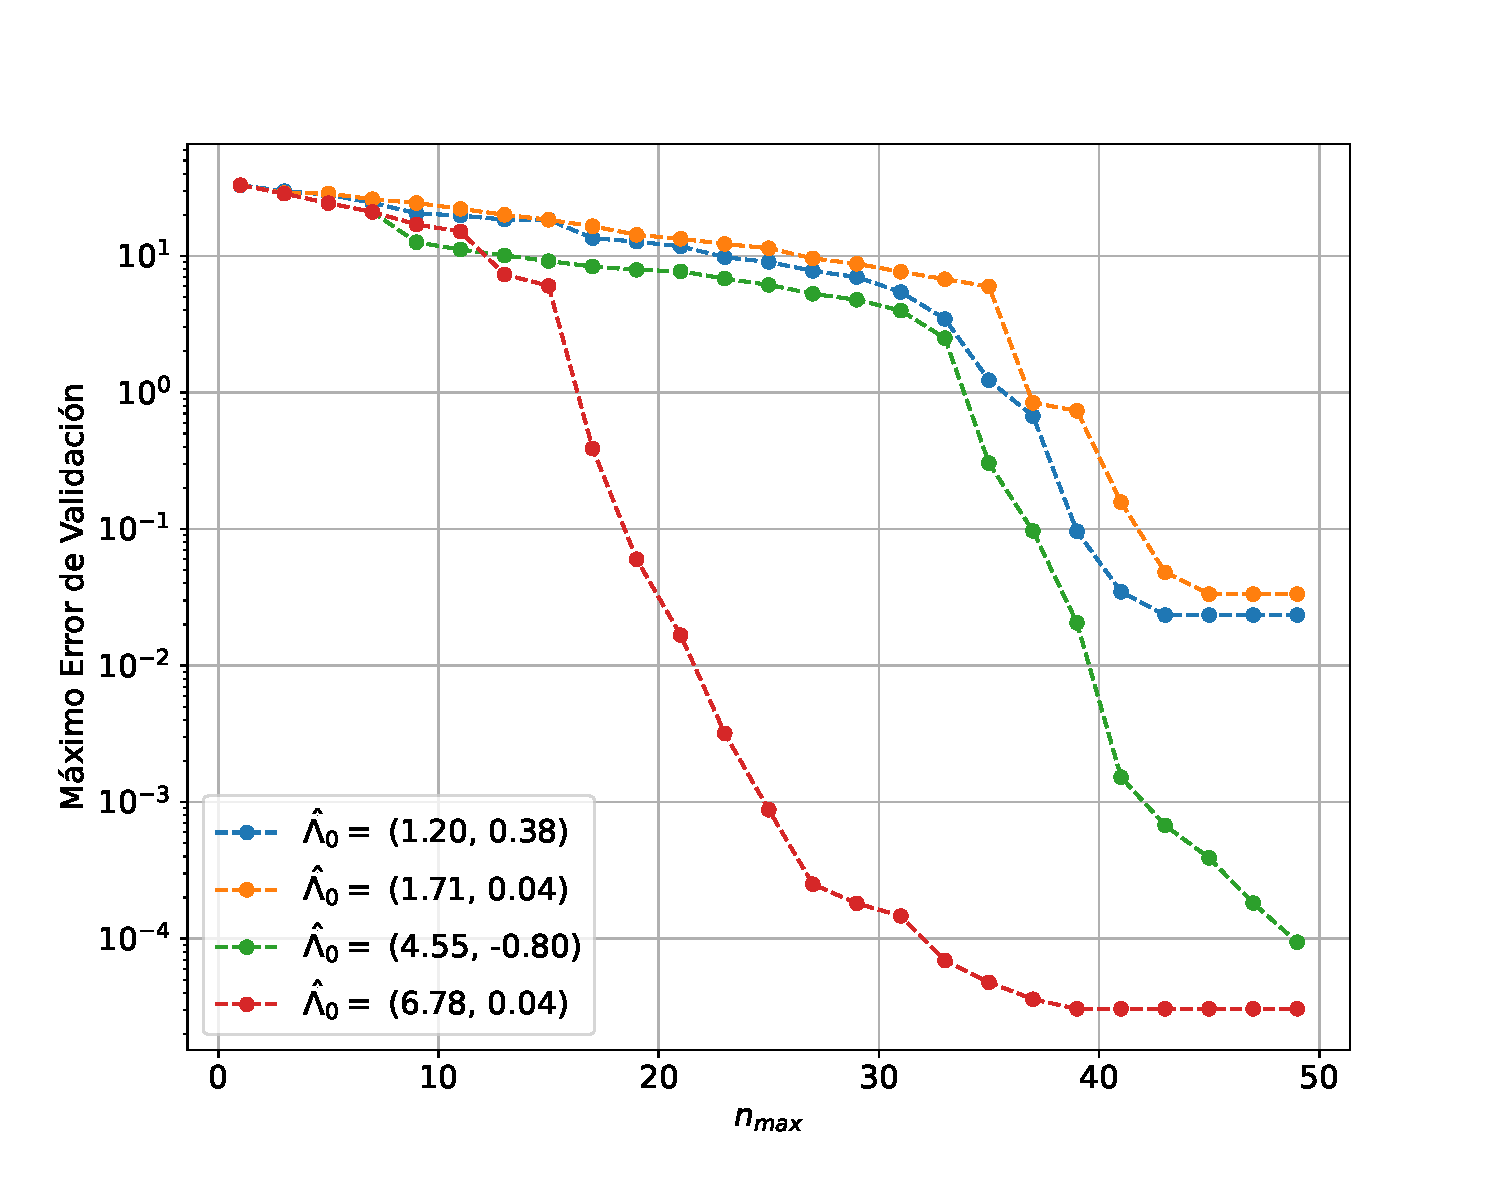
\includegraphics[width=.8\columnwidth ,trim={1.1cm, 1.1cm, 1.2cm, 1.2cm}]{figs/Semillas_v_nmax_2D.pdf}
\caption{Error de validación para diferentes semillas.}
\label{fig:seeds0}
\end{figure}

\begin{itemize}
\item $\bm{\hat{\Lambda}_0}$: la semnilla no es más que el primer parámetro \textit{greedy} de la base global. En cada base local, el primer parámetro \textit{greedy} no es relevante, pero en el caso de las bases \textit{hp-greedy} cada semilla dará lugar a una división diferente del dominio de parámetros. En la figura \ref{fig:seeds0} se puede ver como cuatro semillas diferentes dan lugar a cuatro curvas de error con distinta convergencia. En la figura \ref{fig:seeds_part}, por otro lado, se observa el resultado de la partición del dominio para tres semillas diferentes. En general las semillas que mejor funcionan (con el conjunto de datos utilizado) son las que logran una partición regular del dominio de parámetros.
\end{itemize}



\begin{figure}[h!]
\centering
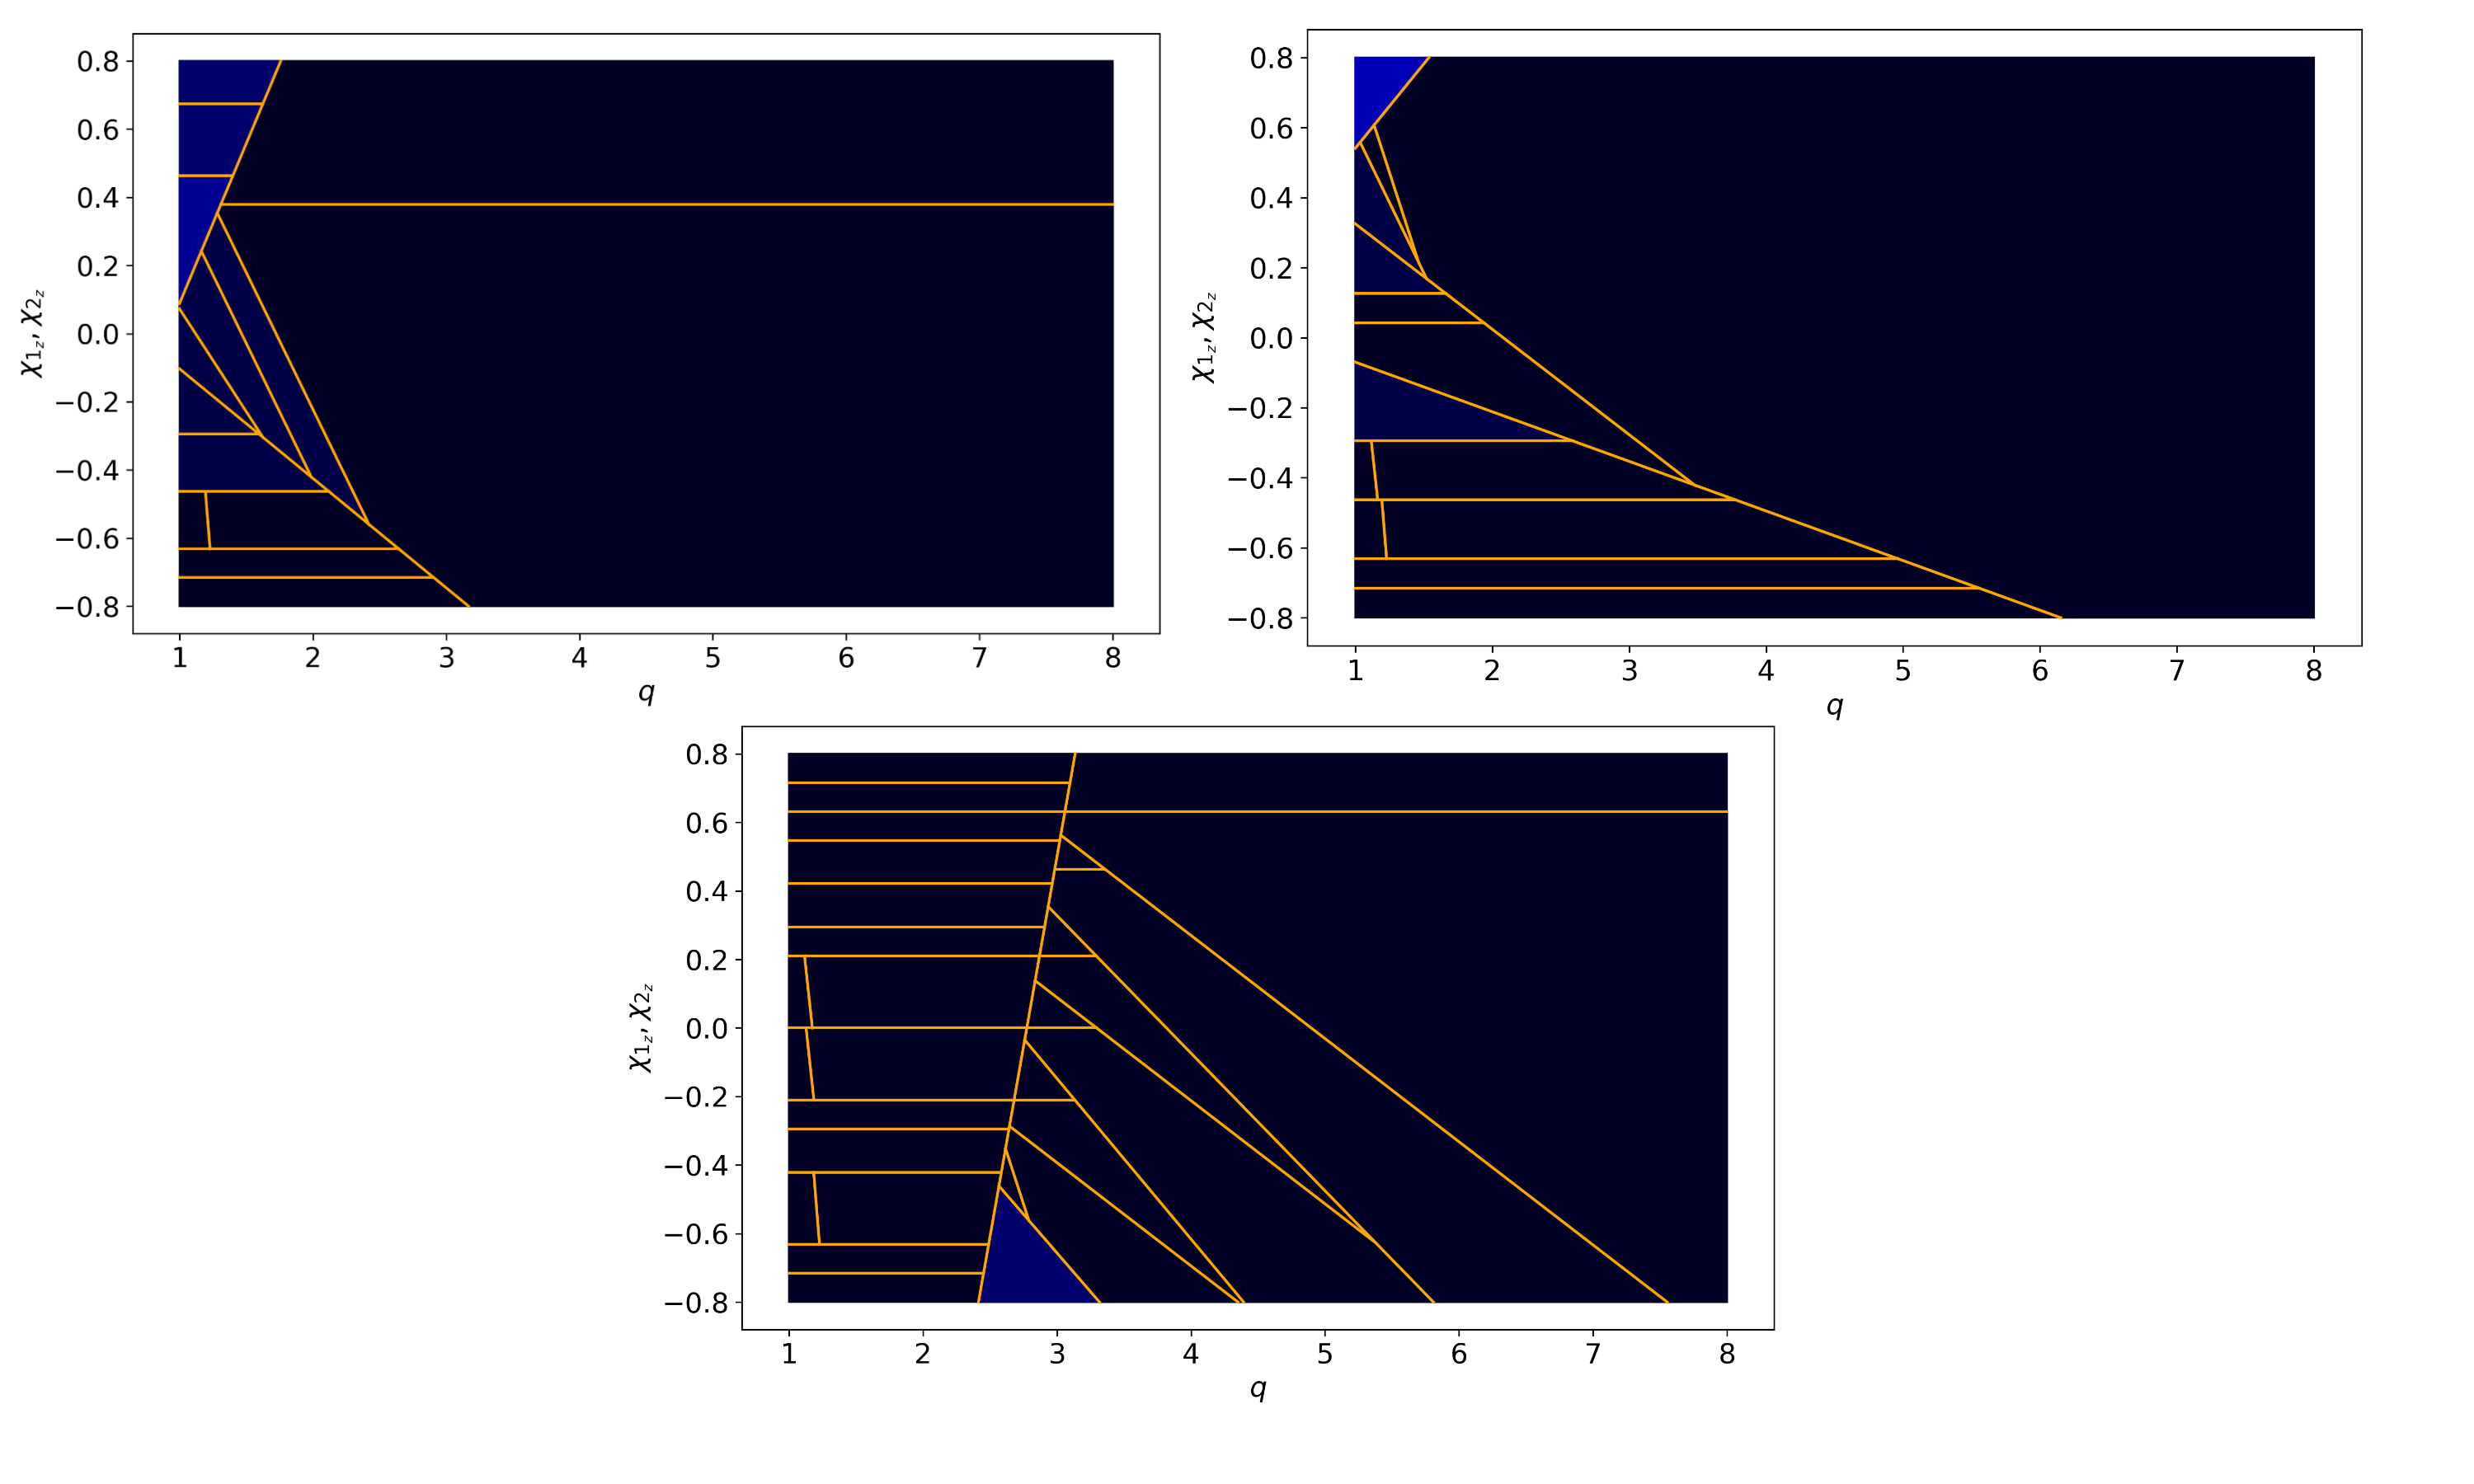
\includegraphics[width=1.05\columnwidth ,trim={1.1cm, 1cm, 1cm, 1.2cm}]{figs/3_semillas_particion.png}
\caption{Partición del espacio de parámetros para tres semillas diferentes; a la izquierda $\hat{\Lambda}_0 = (1.2 \ \ 0.38)$, a la derecha $\hat{\Lambda}_0 = (1.71 \ \ 0.04)$ y al centro $\hat{\Lambda}_0 =(4.55 \ \ -0.8)$.}
\label{fig:seeds_part}
\end{figure}



